\documentclass[conference]{IEEEtran}
\IEEEoverridecommandlockouts
% The preceding line is only needed to identify funding in the first footnote. If that is unneeded, please comment it out.
% Template version as of 6/27/2024

\usepackage{cite}
\usepackage{amsmath,amssymb,amsfonts}
\usepackage{algorithmic}
\usepackage{graphicx}
\usepackage{textcomp}
\usepackage{xcolor}
\def\BibTeX{{\rm B\kern-.05em{\sc i\kern-.025em b}\kern-.08em
    T\kern-.1667em\lower.7ex\hbox{E}\kern-.125emX}}

% Avoid word-breaking
\hyphenpenalty=10000
\exhyphenpenalty=10000

\begin{document}

\title{HSL-Throw: The Hand-Launchable Two-Wheeled Rescue Robot}

\author{\IEEEauthorblockN{Saeed Bazargan}
\IEEEauthorblockA{\textit{Dept. of Computer and Electrical Engineering} \\
\textit{Qazvin Islamic Azad University, Mechatronics Research Lab}\\
Qazvin, Iran \\
0009-0002-9326-4760}
\and
\IEEEauthorblockN{Mohammad Norouzi}
\IEEEauthorblockA{\textit{Dept. of Computer and Electrical Engineering} \\
\textit{Qazvin Islamic Azad University, Mechatronics Research Lab}\\
Qazvin, Iran \\
mh.norouzi@gmail.com}
}
\maketitle

\begin{abstract}
Developing versatile and cost-effective rescue robots is crucial for improving safety and efficiency in hazardous environments where human access is restricted. In response to this demand, we have designed a compact and affordable mobile robot platform, equipped with diverse sensors for easy transport and rapid deployment. This platform supports rescue missions, research, and educational applications, providing semi-autonomous assistance through advanced object detection capabilities. A notable feature of this design is the ability to stream the camera feed from the robot to an external laptop, where object detection is performed using the \mbox{YOLOdotnet framework integrated} with a custom GUI. This approach enhances processing speed and conserves battery life by offloading computationally intensive tasks. With a focus on functionality, accessibility, cost-effectiveness, and open-source design, the platform includes a comprehensive SDK. The electronic system is centered around a 32-bit ARM microcontroller operating FreeRTOS with task scheduling, while a Raspberry Pi Zero 2W board is responsible for wireless communication and environmental sound detection. This paper also explores the ongoing integration of artificial intelligence, currently under development by the MRL Mechatronics Research Lab, enhancing the robot's capabilities.\\
\end{abstract}

\begin{IEEEkeywords}
Rescue Robots, Mobile Robot Platform, Human-Robot Interaction, YOLODotNet, FreeRTOS, ARM Microcontroller.
\end{IEEEkeywords}

\section{Introduction}
Rescue robots are becoming increasingly valuable for search and rescue operations due to their ability to navigate rubble and hazardous environments \cite{Messina2007}. Unlike dogs or human responders, these robots are expendable, making them ideal for initial assessments in dangerous areas. Insights from past rescue missions have highlighted several challenges and limitations in current systems. One major challenge in urban search and rescue operations is disaster environments' unpredictable and highly varied nature. Although numerous solutions have been proposed, none have proven to be both affordable and reliable enough. And reliable enough for widespread adoption across various rescue scenarios. In recent years, significant progress has been made in object detection, particularly with the advancement of deep convolutional neural networks (CNNs). One standout framework in this area is YOLO (You Only Look Once), known for its real-time processing capabilities. In our study, we decided not to perform YOLO processing directly on the Raspberry Pi \cite{Yao2022}; instead, the camera feed is streamed to an external laptop. A custom GUI, developed in C\#, leverages the YOLOdotnet framework to boost processing speed and reduce the robot's battery consumption. The robot operates more efficiently by offloading computationally intensive tasks to the laptop while maintaining strong object detection capabilities. This paper examines previous rescue missions that utilized rescue robots, focusing on the challenges of identifying trapped individuals or objects in complex environments. We explore the benefits of using deep learning models like YOLOdotnet to improve detection capabilities in rescue scenarios.
Additionally, we introduce the rescue robot platform, HSL, and provide a review of similar systems, such as Recon Scout and iRobot FirstLook \cite{ReconRobotics_ScoutXL, ReconRobotics_ThrowbotXT}. The following sections will delve deeper into the performance and capabilities of existing rescue robot platforms (as shown in Figure.~\ref{fig_First}). Finally, we will give an overview of the HSL robot system and describe how YOLOdotnet is integrated for object detection.

\begin{figure}[htbp]
\centerline{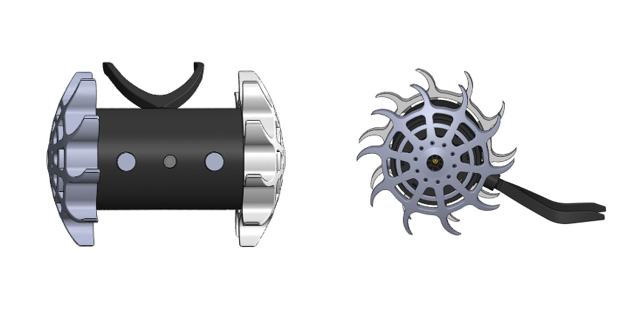
\includegraphics[width=0.5\textwidth]{Fig_First.PNG}}
\caption{HSL-Throw robot CAD view.}
\label{fig_First}
\end{figure}

\section{Existing Rescue Mobile Robot Platforms}
The system described in this paper is designed to meet the requirements of a portable and deployable rescue robot. In recent decades, numerous mobile rescue robot platforms have been developed, emphasizing the importance of rescue and recovery systems for facilitating effective interaction between artificial intelligence and the environment. We aim to create a platform suitable for research, education, and enhancement, focusing on simplicity \cite{Mathew2014, Karimi2017}. To achieve these objectives, a robust hardware setup with diverse sensors and a modular, programmable design is essential. These features enable researchers to utilize the platform in rescue operations, training sessions, AI laboratories, and various real-world robotics applications. In this context, several robotic platforms have been specifically designed for rescue, research, and educational purposes within the field of rescue robotics. One of the most widely recognized platforms is the Recon Scout, shown in Figure~\ref{Fig_iRobotAndRecon}. While this robot is not ideally suited for high-precision rescue tasks in real environments due to its fully manual control by human operators, it remains applicable in other scenarios. Furthermore, the project presented here has developed a robotic platform that supports wireless remote communication and connectivity, allowing it to perform tasks previously challenging for most mobile robots, such as deployment in harsh conditions and waterproof operation.

\begin{figure}[htbp] 
    \centerline{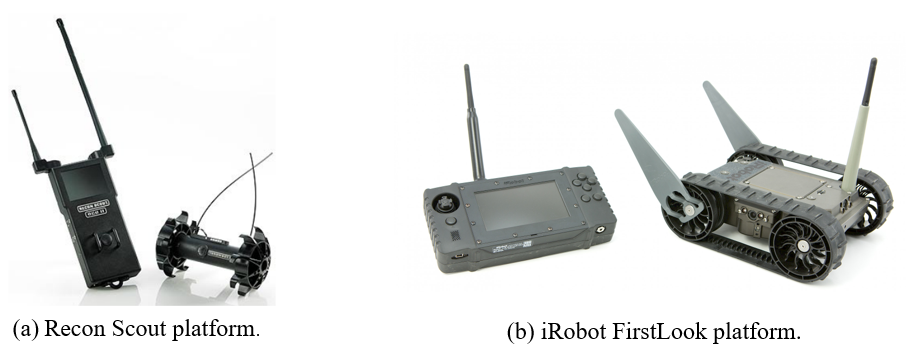
\includegraphics[width=0.5\textwidth]{Fig_iRobotAndRecon.PNG}} 
    \caption{Examples of existing rescue mobile robot platforms.} 
    \label{Fig_iRobotAndRecon} 
\end{figure}

Additionally, the IRobot FirstLook platform \cite{iRobot_FirstLook} was reviewed (Figure~\ref{Fig_iRobotAndRecon}), capable of performing tasks on a laboratory scale. This platform can be utilized in research laboratories and technical labs, with the potential for experiences gained to be applied to industrial contexts. However, this robot is not open-source, and its cost is relatively high for students and research labs. The study emphasized the need for a compact and affordable general-purpose rescue robot for initial response. Consequently, a robust, low-cost, and portable robotic platform is currently in development, intended as a primary investigative tool in any disaster scenario. This design follows Jacoff's recommendation that the entire robotic system and necessary tools should be operable by a single operator \cite{Murphy2008}. The robot can be deployed by being thrown or dropped from heights of up to 5 meters and is affordable enough to be considered disposable or replaceable. This ensures that rescue operations can begin without waiting for more advanced and specialized robots to arrive on the scene.

\section{System Overview}
The platform described in this paper is designed to fulfill the requirements of a portable and throwable rescue robotic system. The HSL platform consists of three main components: the mechanical structure, electronic components, and software architecture. The mechanical structure is divided into two parts: the robot's body and the movement system. The body is made of 3D-printed PLA, with a cylindrical shape, measuring 13 cm in height and 16 cm in length. The HSL's movement relies on a two-wheel robotic system. In the electronics section, the HSL consists of two main components. The first is a Raspberry Pi board with a 64-bit ARM processor, featuring Cortex-A53 architecture. It operates at a frequency of 1 GHz and runs on the Debian operating system, handling tasks related to receiving and transmitting sensor data, including images and audio, to the server. The second component is a processor based on a 32-bit ARM microcontroller with Cortex-M3 architecture, known as the STM32f103CB \cite{CarmineNoviello2022}. It operates at a frequency of 72 MHz, has 20 KB of RAM, and 128 KB of flash memory, and runs under the FreeRTOS operating system \cite{GUAN201619}. This unit can control and access all sensor and actuator data, such as the Inertial Measurement Unit (IMU), current, voltage, and actuator encoder. To send this information to the server, the data is first transmitted to the Raspberry Pi using the UART unit, which operates in half-duplex mode \cite{teimouri2018mrl}, and then the Raspberry Pi forwards it to the server based on its assigned tasks. Each input/output module can be activated or deactivated in real time by sending operational commands. This method allows the use of high-frequency sensors for specific tasks and the ability to power certain sensors/motors at a desired frequency, turn some entirely off, or place them in standby mode, especially when executing complex tasks. This capability can be utilized in sensor selection algorithms and contributes to energy efficiency. The block diagram of the HSL, depicted in Figure~\ref{Fig_BlockDiagram}, can help researchers implement their algorithms more quickly.

\begin{figure}[htbp] 
    \centerline{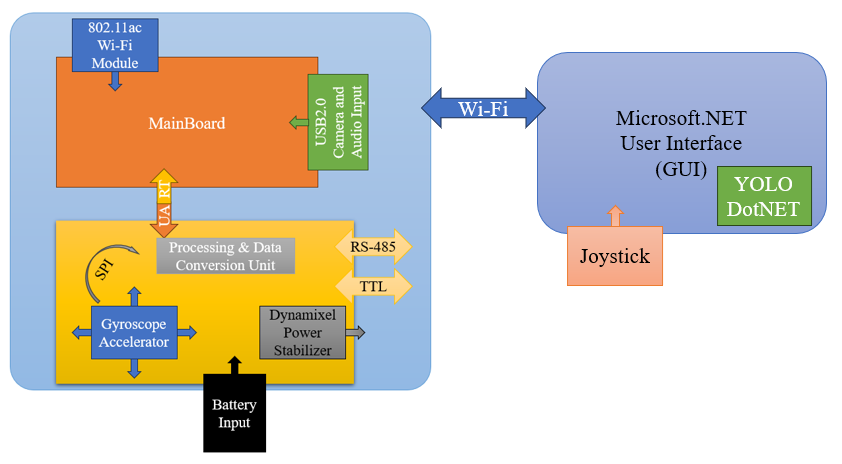
\includegraphics[width=0.5\textwidth]{BlockDiagram.PNG}} 
    \caption{Block diagram of the electronic system embedded in the HSL-Throw} 
    \label{Fig_BlockDiagram}
\end{figure}

In the HSL platform, all I/O requests are handled using the FreeRTOS operating system to ensure reliable and secure information. Most primary processing, such as filtering inertial system sensor data and power management, is performed in this unit. This process is designed to collect and update all necessary information via the operating system, and if a request is made, the corresponding responses are transmitted. The management system that oversees data collection and motor update commands can reduce power consumption by controlling each module's reading frequency and activity. Additionally, after completing all operations and sending them to the server, the user can select unique features. For instance, they can manage the YOLO algorithm's usage \cite{Han2021}, choose the color format of received images, and control the activation or deactivation of audio. The robot is user-controlled via a USB PlayStation joystick. To correct for wheel deviations and navigate rough terrain, a PID controller fine-tunes the robot's movements. Furthermore, when employing the YOLO algorithm, the user can detect individuals or objects that might otherwise be missed due to disturbances.

\section{HSL-Throw Construction}
In this section, we introduce the design of the HSL robot. The implementation of the robot has been designed to be as simple as possible, and its material is plastic, which offers advantages such as low cost, appropriate weight, and good appearance. The tail connected at the outer angle of the robot serves as a handle for easier carrying and assists in throwing. Upon impact, the robot's wheels absorb a significant portion of the impact energy, protecting the internal components. Due to the hazards present in rescue environments, there is a risk of the rescue robot becoming irreversibly oriented towards the operator, as the robot stores the distance traveled in various directions during movement. In general, designers of mobile robots have divided the design problem into several subsets \cite{braunl2006embedded}, such as:
\begin{itemize}
    \item Sensing
    \item Task planning and execution
    \item Motion control
\end{itemize}

We have tried to avoid these approaches and instead focus on important factors, such as sensor and module integration, precise mechanical design, and eliminating hardware noise for sensors, to achieve an optimized structure. To this end, instead of using a self-balancing robot motion system, a tail has been utilized to maintain balance, which also significantly aids in overcoming obstacles up to 12 centimeters in height.

\subsection{Motion System}
Dynamixel actuators have been used for years in the production and applications of mobile robots. The HSL platform features a two-wheel system that allows it to move independently along each axis. An omnidirectional robot can move straight from point A to point B while simultaneously rotating along the line to reach its destination with the correct orientation. Two parameters of electric actuators are very important in the design and construction of wheeled robots: first, output torque, and then the no-load speed of the motor, which directly affects the acceleration and speed of the robot. The wheels designed for the HSL platform have a diameter of 15 centimeters, and the maximum adjustable speed in Dynamixel is 60 RPM. Considering the robot's geometry, the distance traveled and orientation of the robot can be calculated as follows:

\begin{equation}
d = \frac{(RPM \times \text{wheel diameter} \times \pi)}{60 \times t} \label{eq:distance}
\end{equation}

where \( d \) is the distance traveled.

\begin{equation}
x_{\text{new}} = x_{\text{old}} + \frac{r \times (\omega_R + \omega_L)}{2 \times \cos(\theta) \times \Delta t}
\end{equation}
\begin{equation}
y_{\text{new}} = y_{\text{old}} + \frac{r \times (\omega_R + \omega_L)}{2 \times \sin(\theta) \times \Delta t}
\end{equation}
\begin{equation}
\theta_{\text{new}} = \theta_{\text{old}} + \frac{r \times (\omega_R - \omega_L)}{L \times \Delta t}
\end{equation}

Also,
\begin{itemize}
    \item \( r \) is the radius of the wheels.
    \item \( \omega_R \) and \( \omega_L \) are the angular velocities of the right and left wheels, respectively.
    \item \( \theta \) is the orientation of the robot.
    \item \( \Delta t \) is the time increment.
    \item \( L \) is the wheelbase (the distance between the centers of the two wheels).
\end{itemize}

Finally, the characteristics of the locomotion system are shown in Table 1:
\begin{table}[htbp]
\centering
\caption{HSL Locomotion Specifications}
\begin{tabular}{|l|l|}
\hline
\textbf{Characteristics}   & \textbf{HSL Locomotion Specification} \\ \hline
Shaft encoder resolution   & 4096 [pulse/rev]                      \\ \hline
Max linear speed           & 39 cm/s                               \\ \hline
Wheel size                 & 15 cm                                 \\ \hline
No Load Speed              & 50 RPM                                \\ \hline
\end{tabular}
\label{tab:hsl_locomotion}
\end{table}

\subsection{Central Controller}
A Raspberry Pi Zero 2W, as a compact and cost-effective processor, enables the implementation of various computationally simple programs. While Raspberry Pi boards may have limited flexibility compared to other processing systems (such as embedded computers) due to their inherent system constraints, they are ideal for creating simple electronic devices that do not require significant modifications over time. These boards are capable of processing diverse data, transmitting signals, and sending information to computers or other devices. A 32-bit microcontroller is also used as an additional processor in this robot, which can process and filter sensor data, send control signals to actuators, and relay information to computers or other devices. This processing unit includes an STM32F103CB microcontroller and the firmware is developed under standard HAL drivers \cite{STM32_ReferenceManual}, customized for the HSL on a printed circuit board (PCB). The HSL platform consists of various modules that can communicate via communication buses like SPI, which is used to read data from the Inertial Measurement Unit (IMU) and for filtering via a complementary filter \cite{allgeuer2014robust}. The serial TTL and RS485 buses are also used for communication with Dynamixel actuators. The general specifications of the HSL platform are shown in Table 2.

\begin{table}[htbp]
\centering
\caption{Specifications of HSL-Throw Robot}
\begin{tabular}{|p{3cm}|p{5cm}|}
\hline
\textbf{Component}         & \textbf{Specification} \\ \hline
Servo Motors               & MX-28 Dynamixel      \\ \hline
Sensors                    & MPU-9250, Logitech C920 \\ \hline
Embedded PC Board          & Sub Controller: Custom-built controller; Main Controller: Raspberry Pi Zero 2W \\ \hline
Battery                    & Li-Po 3-Cell 3500mAh    \\ \hline
\end{tabular}
\label{tab:hsl_locomotion}
\end{table}

\subsection{Rotary Encoder Functionality}
A rotary encoder converts rotational position into an analog or digital electronic signal. The Hall Sensor encoder used in Dynamixel actuators, known as AS5045, operates with a micro-magnet directly attached to the motor shaft to measure rotational speed and wheel direction. This 12-bit encoder provides a resolution of 4096 pulses per revolution, as shown in Table 1.

\subsection{Software architecture and SDK}
One of the primary design goals of the HSL platform is to maximize accessibility for researchers. This goal has been achieved in two main aspects: simplified access to the hardware layer (including sensors, motion control, and communications) and compatibility with general software libraries through an expandable software structure. As explained in previous sections, the WeeMiK hardware platform includes multiple sensors, actuators, and communication systems. At the low-level hardware system, many of these modules interact with and are managed by the STM32 microcontroller. The provided software architecture and SDK form a real-time operating system (RTOS)-based framework for the HSL-Throw robot, designed for applications in mapping, localization, and autonomous navigation in both real and engineered environments. The RTOS framework serves as a hard real-time software environment for scheduling operational devices and robots. Similar to the hardware design, all features of the software and control system will be released under an open-source license and made available on a GitHub repository. Documentation, tutorials, and example projects will also be maintained on this website.

\section{Experimental Results} 
To test and evaluate the capabilities of the HSL platform, we conducted two sets of experiments. The first set aimed to test and identify the movement system and obstacle detection for individuals, along with the path-planning capabilities of the HSL platform. In these tests, we used sensor fusion algorithms combining data from the inertial navigation system, odometer, and object detection. Our first experiment demonstrates the suitability of the HSL platform as a mobile rescue robot capable of automatically detecting objects or individuals (Figure~\ref{Fig_HSL-Throw}).

\begin{figure}[htbp] 
    \centerline{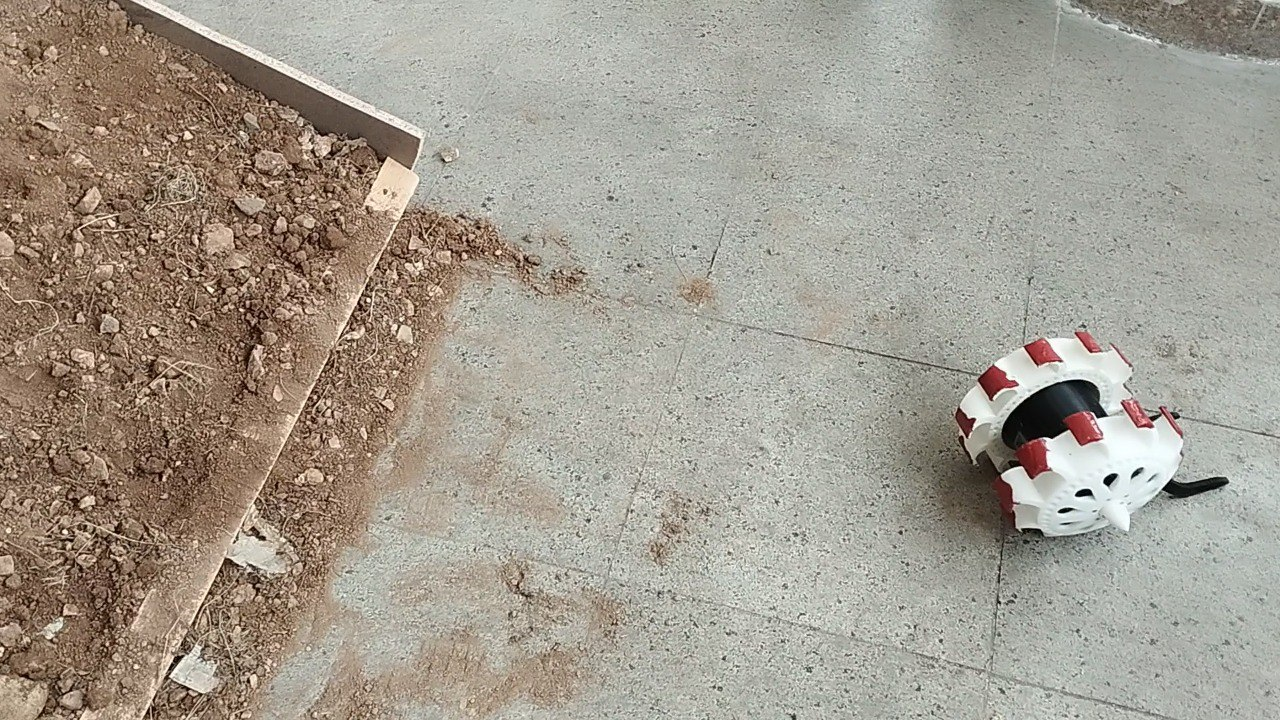
\includegraphics[width=0.45\textwidth]{HSL-Throw.png}} 
    \caption{HSL-Throw robot platform in a simulated environment}
    \label{Fig_HSL-Throw} 
\end{figure}

The second experiment assessed power management, long-range wireless communication, and waterproof capabilities. To evaluate platform performance, we measured communication accuracy and power consumption necessary for performing rescue operations. The test area was structured as shown in Figure 5, where the HSL was able to maintain communication with the operator over a distance of up to 220 meters, position itself in hazardous locations, send information back to the user, and finally return to its starting point based on the path it followed if directed to do so by the operator.

\section{Conclusion}
This paper presented the design concepts, development, and applications of the HSL-Throw rescue mobile robot. Our primary aim was to create a versatile, low-cost robotic platform suitable for real-world rescue operations, with a significantly lower cost than other available robots, such as the Recon Scout and IRobot FirstLook. This platform is intended not only for rescue operations but also for expanding research and educational applications involving artificial intelligence and multi-agent functionality. A key requirement for achieving a low-cost robot capable of use across such diverse fields is that it must be highly configurable and modular. Therefore, HSL-Throw was designed with numerous sensors and a flexible movement system that allows optional reconfiguration based on a modular I/O structure and powerful layered management. While certain components are still under development, the work completed thus far demonstrates a reliable proof-of-concept. The platform is simple enough to be easily replaceable, yet robust enough for deployment through throwing. However, full integration and testing of the current system are still pending, and thus, these will be the focus of future work. Testing the system in a real-world environment—whether in an actual disaster or a simulated setting—will provide invaluable insights. This data will guide future development steps and highlight specific areas for improvement. Following the recommendations of Murphy and Casper, real-time image processing could be implemented to facilitate the detection of objects associated with victims, such as body parts, watches, and glasses.

\bibliographystyle{IEEEtran}
\bibliography{References}

\end{document}
